%%%%%%%%%%%%%%%%%%%%%%%%%%%%%%%%%%%%%%%%%%%%%%%%%%%%%%%%%%%%%%%%%%%%%%
%%                     Annotation
%%%%%%%%%%%%%%%%%%%%%%%%%%%%%%%%%%%%%%%%%%%%%%%%%%%%%%%%%%%%%%%%%%%%%%

\section{Glyph: \glyph{Annotation}}
\label{sec:annotation}

\SBGNERLone defines a glyph to add additional information to a map, that does not modify the semantic of the graph. This glyph can be used to add free text, or links to external information.

\begin{glyphDescription}

\glyphSboTerm SBO:0000550 ! annotation.

\glyphContainer An \glyph{annotation} is represented by a rectangular container with a folded corner, as illustrated in \fig{annotation}. This container is linked to the annotated element with a callout. The link ends up on the border of the annotated element.

\glyphLabel An \glyph{annotation} contains information placed in an unbordered box containing a string of characters.  The characters can be distributed on several lines to improve readability, although this is not mandatory.  The label box must be attached to the center of the container. The label may spill outside of the container. 

\glyphAux An \glyph{annotation} does not carry any auxiliary unit.
\end{glyphDescription}

\begin{figure}[H]
  \centering
  \includegraphics[scale = 0.3]{images/annotation}
  \caption{The \ER glyph for \glyph{annotation}.}
  \label{fig:annotation}
\end{figure}

\begin{figure}[H]
  \centering
  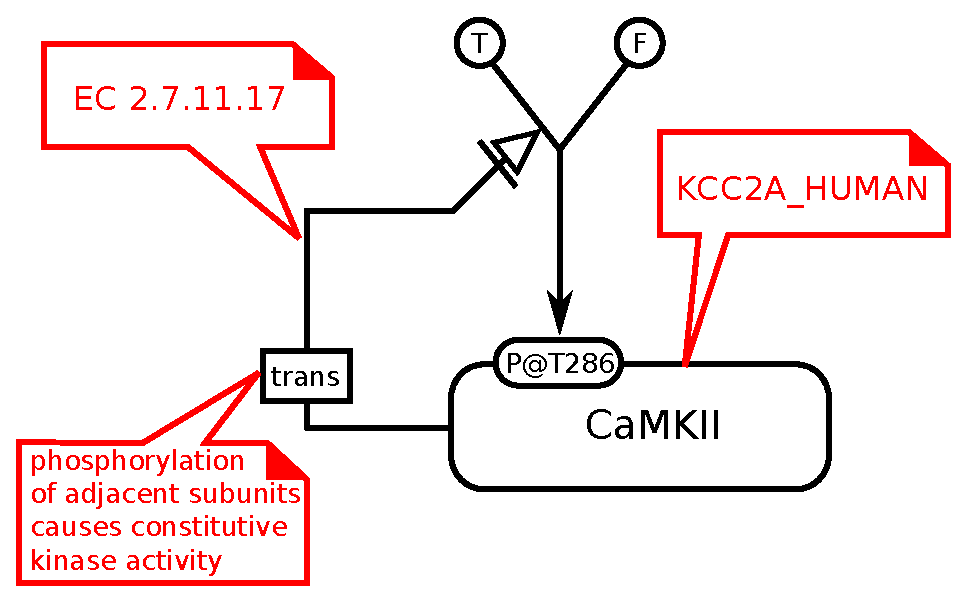
\includegraphics[scale = 0.5]{examples/ex-annotation}
  \caption{Example of \glyph{annotations} adding information to the description of the trans-phosphorylation of CaMKII.}
  \label{fig:ex-annotation}
\end{figure}

%\normalcolor
